\documentclass{beamer}
\usetheme{Warsaw}

\usepackage[utf8]{inputenc}
\usepackage{fancybox}
\usepackage{multimedia} 
\usepackage{subfig}
\usepackage{amsmath}
\usepackage{hyperref}
\hypersetup{
    colorlinks=true,     
    urlcolor=blue
}
\setbeamertemplate{footline}[frame number]

\usepackage[all]{xy}
\begin{document}


\title[Stochastik] % (optional, only for long titles)
{Stochastik für Informatiker
\\
\includegraphics[scale=0.5]{img/craps}
}
\subtitle{}
\author[Dr. Johannes Riesterer] % (optional, for multiple authors)
{Dr.  rer. nat. Johannes Riesterer}

\date[KPT 2004] % (optional)
{}

\subject{Stochastik}

\frame{\titlepage}




\begin{frame}
    \frametitle{Verteilungen}
\framesubtitle{}

\begin{block}{Gleichverteilung}
Die Gleichverteilung $U{(a,b)}$ auf einem Intervall $(a,b) \subset \mathbb{R}$ ist definiert durch
\begin{align*}
& \text{Dichte: } f (x) : = \frac{1_{(a,b)}}{|b-a| } \\
& \Rightarrow \text{Verteilung: } F (x) =  P_f( (-\infty, x))  =  \int_{-\infty}^{x} \frac{1_{(a,b)}}{|b-a|} dt\\\
& = \begin {cases} 0 \text{ für } x \leq a \\   \frac{x-a}{|b-a|} \text{ für } a \leq x \leq b \\ 1 \text{ für }  x \geq b \\  \end{cases}
\end{align*}
\end{block}

 \end{frame}

\begin{frame}
    \frametitle{Verteilungen}
\framesubtitle{}

\begin{figure}[htp]
      \centering
    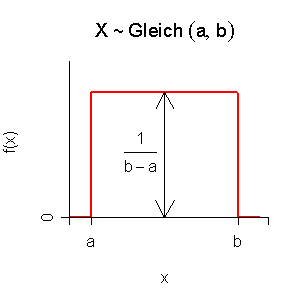
\includegraphics[width=0.42\textwidth]{img/gleichverteilung1}
    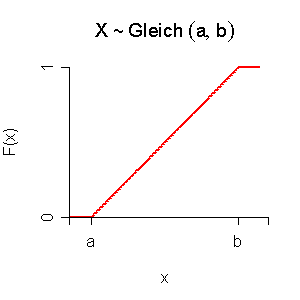
\includegraphics[width=0.42\textwidth]{img/gleichverteilung2}
      \caption{Quelle: Wikipedia}
\end{figure}
 \end{frame}




\begin{frame}
    \frametitle{Verteilungen}
\framesubtitle{}

\begin{block}{Gleichverteilung}
Sei $X \sim $U(a,b).
\begin{align*}
& \mathbb{E}(X) =\int\limits_{-\infty}^\infty x \cdot f(x)\,dx = \frac 1{b-a}\int\limits_a^b x\cdot 1\,dx = \frac 12\frac{b^2-a^2}{b-a} = \frac{a+b}2 \\
& \mathbb{V}(X) = \operatorname{E}(X^2) - \left({\operatorname{E}(X)} \right)^2  = \frac{1}{b - a}\int\limits_a^b {x^2 \cdot 1\,dx}  - \left( {\frac{a + b}{2}} \right)^2  \\
 & = \frac{1}{3}\frac{b^3  - a^3}{b - a} - \left( {\frac{a + b}{2}} \right)^2 \\
    &= \frac{1}{12}\left( {4b^2  + 4ab + 4a^2  - 3a^2  - 6ab - 3b^2 } \right) = \frac{1}{12}(b - a)^2
\end{align*}
\end{block}
 \end{frame}



\begin{frame}
    \frametitle{Verteilungen}
\framesubtitle{}

\begin{block}{Normalverteilung}
Die Normalverteilung $N{(\mu,\sigma^2)}$ auf $\mathbb{R}$ ist definiert durch
\begin{align*}
& \text{Dichte: } f (x) : = \frac 1{\sigma \sqrt{2\pi}}e^{- \frac {1}{2} (\frac{x- \mu}{ \sigma})^2} \\
&  \Rightarrow \text{Verteilung: } F(x) = N{(\mu,\sigma^2)}(-\infty , x) =  \int_{-\infty}^{x}  \frac 1{\sigma \sqrt{2\pi}}e^{- \frac {1}{2} (\frac{t- \mu}{ \sigma})^2}dt\\
\end{align*}

\end{block}
 \end{frame}



\begin{frame}
    \frametitle{ Verteilungen}
\framesubtitle{}
\begin{figure}[htp]
      \centering
    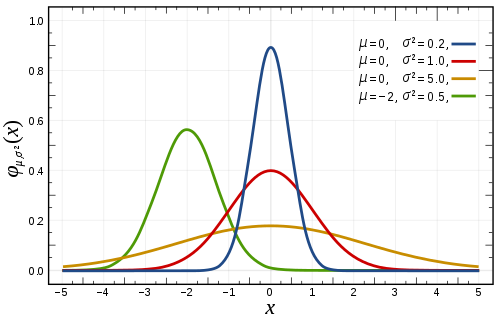
\includegraphics[width=0.45\textwidth]{img/normal}
    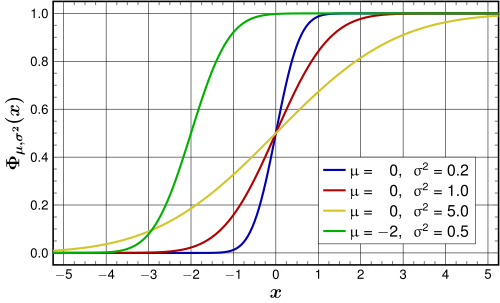
\includegraphics[width=0.45\textwidth]{img/normaldist}
      \caption{Quelle: Wikipedia}
\end{figure}

 \end{frame}


\begin{frame}
    \frametitle{Verteilungen}
\framesubtitle{}

\begin{block}{Normalverteilung}
Sei $X \sim N(\mu, \sigma^2)$.
\begin{align*}
& \mathbb{E}(X) = \mu \\
& \mathbb{V}(X) = \sigma^2
\end{align*}
\end{block}
 \end{frame}



\begin{frame}
    \frametitle{ Verteilungen}
\framesubtitle{}

\begin{block}{Poissonverteilung}
Die Poissonverteilung  $Pois (\lambda)$ auf $\mathbb{N}_{\geq 0}$ ist definiert durch
\begin{align*}
& P_\lambda (k) = \frac{\lambda^k}{k!}\, \mathrm{e}^{-\lambda} \\
& \Rightarrow F_{\lambda}(n)=\sum_{k=0}^n P_\lambda (k) = \mathrm{e}^{-\lambda} \sum_{k=0}^n \frac{\lambda^k}{k!}
\end{align*}
\end{block}
\begin{figure}[htp]
      \centering
    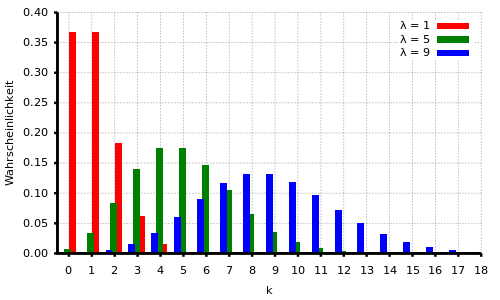
\includegraphics[width=0.55\textwidth]{img/Poisson}
      \caption{Quelle: Wikipedia}
\end{figure}
 \end{frame}



\begin{frame}
    \frametitle{ Verteilungen}
\framesubtitle{}

\begin{block}{Poisson Verteilung}
Die Poisson Verteilung beschreibt das Auftreten von seltenen Ereignissen und spielt bei Zählprozessen eine wichtige Rolle.
\end{block}
\begin{block}{Poisson Verteilung}
$X\sim Pois (\lambda)$ 
\begin{align*}
& \mathbb{E}(X) = \lambda \\
& \mathbb{V}(X) = \lambda
\end{align*}
\end{block}
 \end{frame}


\begin{frame}
    \frametitle{Verteilungen}
\framesubtitle{}

\begin{block}{Bernoulliverteilung}
Die Bernoulliverteilung  Für $\Omega = \{ 0, 1\}$ und $p \in [0,1]$ ist definiert durch
\begin{align*}
P (\omega) = p^{\omega} (1-p)^{1 -\omega}
\end{align*}
\end{block}

\begin{block}{Beispiele}

\begin{itemize}
\item Werfen einer Münze: Kopf (Erfolg), $p=1/2$, und Zahl (Misserfolg), $q=1/2$.
\item Werfen eines Würfels, wobei nur eine 6 als Erfolg gewertet wird: $p=1/6, q=5/6$.
\item Qualitätsprüfung (einwandfrei, nicht einwandfrei).
\item Betrachte sehr kleines Raum/Zeit-Intervall: Ereignis tritt ein $(p \gtrapprox 0)$, tritt nicht ein $(q\lessapprox 1)$.
\end{itemize}

\end{block}
 \end{frame}




\begin{frame}
    \frametitle{ Verteilungen}
\framesubtitle{}

\begin{block}{Binomialverteilung}
$B(k,  p,n)= \binom nk p^k (1-p)^{n-k} $
\end{block}
\begin{block}{Binomialverteilung}
$X_1, \cdots ,X_n \sim B \Rightarrow \sum X_i  \sim B$
\end{block}

\begin{figure}[htp]
      \centering
    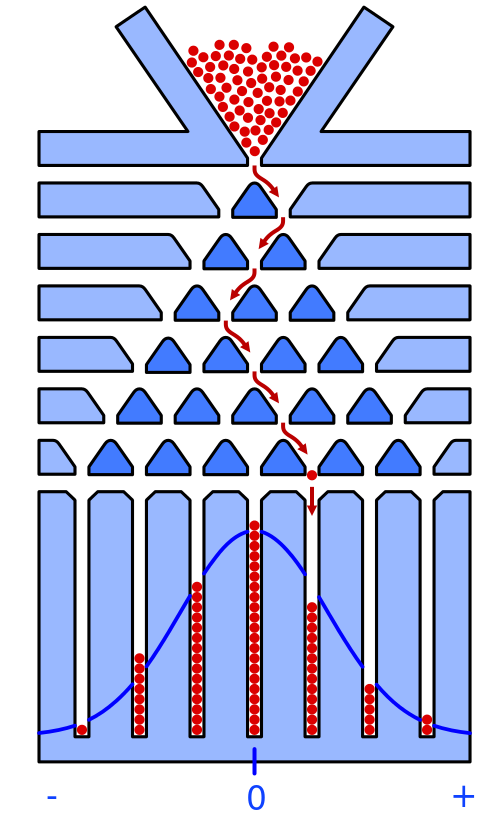
\includegraphics[width=0.25\textwidth]{img/Galton}
      \caption{Quelle: Wikipedia}
\end{figure}
 \end{frame}




\begin{frame}
    \frametitle{Zentraler Grenzwertsatz}
\framesubtitle{}

\begin{block}{Motivation}
Welche Verteilung hat das arithmetische Mittel $S_n:= \frac{1}{n} \sum_{i=1}^n X_i$ für $n \to \infty$?
\end{block}
\begin{block}{Motivation}
Wie und gegen was konvergiert $P_{S_n}$ für $n \to \infty$?
\end{block}

 \end{frame}



\begin{frame}
    \frametitle{Zentraler Grenzwertsatz}
\framesubtitle{}

\begin{block}{Konvergenz von W-Maßen}
Was bedeutet Konvergenz einer Folge von Wahrscheinlichkeitsmaßen?
\end{block}
\begin{block}{Inspiration: Gleichmäßige Konvergenz von Funktionen}
Eine Folge von Funktionen $f_n: A \subset \mathbb{R}^n \to \mathbb{R}$ konvergiert gleichmäßig gegen eine Funktion $f$, falls 
\begin{align*}
\lim_{n \to \infty} ||f_n(x) -f(x) || = 0
\end{align*}
für alle $x \in A$.
\end{block}

 \end{frame}

\begin{frame}
    \frametitle{Allgemeine Wahrscheinlichkeitsräume/Nachtrag}
\framesubtitle{}

\begin{block}{Konvergenz von W-Maßen}
Sei $(\Omega, \mathcal{A})$ ein Wahrscheinlichkeitsraum und $P_n : \Omega \to [0,1]$ eine folge von Wahrscheinlichkeits-Maßen. Die Folge konvergiert gegen
das Wahrscheinlichkeits-Maß $P: \Omega \to [0,1]$, falls 
\begin{align*}
\lim_{n \to \infty} \int_\Omega f dP_n = \int_\Omega f dP
\end{align*}
für alle messbaren Funktionen $f: \Omega \to \mathbb{R}$.
\end{block}
 \end{frame}

\begin{frame}
    \frametitle{Highlight}
\framesubtitle{}
\begin{figure}[htp]
      \centering
    
\includegraphics[width=0.9\textwidth]{img/firework}
\end{figure}
 \end{frame}


\begin{frame}
    \frametitle{Zentraler Grenzwertsatz}
\framesubtitle{}


\begin{block}{Zentraler Grenzwertsatz}
Sei $(\Omega, \mathcal{A}, P)$ ein Wahrscheinlichkeitsraum und $X_n :  \Omega \to \mathbb{R}$  eine folge stochastisch unabhängiger, identisch verteilter, reeller Zufallsvariablen mit $\mathbb{E}(X_n) = \mu$ und $\mathbb{V}(X_n)= \sigma^2$. Dann gilt für das arithmetische Mittel $S_n:= \frac{1}{n} \sum_{i=1}^n X_i$
\begin{align*}
P_{ \frac{\sqrt{n}}{\sigma} (S_n-\mu)} \to P_{N(0,1)}
\end{align*}
wobei $ P_{N(0,1)}$ das Wahrscheinlichkeits-Maß mit der Dichte $ \frac {1}{ \sqrt{2\pi}}e^{- \frac {1}{2} x^2}$ ist.
\end{block}

 \end{frame}



\begin{frame}
    \frametitle{Zentraler Grenzwertsatz}
\framesubtitle{}

\begin{block}{Erzeugende Funktion}
Sei $(\Omega, \mathcal{A}, P)$ ein Wahrscheinlichkeitsraum und $X :  \Omega \to \mathbb{R}$  eine reelle Zufallsvariable. Dann heißt die Funktion 
\begin{align*}
\psi_X(t) := \mathbb{E}(e^{tX}), \; t \in I \subset \mathbb{R}
\end{align*}
erzeugende Funktion zu $X$ bzw. $P_X$.
\end{block}

\begin{block}{Stetigkeitssatz von  Lévy }
Sei $(\Omega, \mathcal{A}, P)$ ein Wahrscheinlichkeitsraum so wie  $X$ und $X_n :  \Omega \to \mathbb{R}$   reelle Zufallsvariablen mit erzeugenden Funktionen $\psi$ und $\psi_{n}$. Dann gilt:
\begin{align*}
\psi_n \to \psi \Rightarrow P_{X_n} \to P_X 
\end{align*}
\end{block}

 \end{frame}


\begin{frame}
    \frametitle{Zentraler Grenzwertsatz}
\framesubtitle{}

\begin{block}{Stetigkeitssatz von Levy}
Mit $\varphi_{X} := \mathbb{E}(e^{i tx})$  ist $\varphi _{X}(-it)=\psi_{X}(t)$ und der Stetigkeitssatz von Levy folgt aus dem Umkehrsatz.
\end{block}
 \end{frame}




\begin{frame}
    \frametitle{Zentraler Grenzwertsatz}
\framesubtitle{}
\begin{block}{Eigenschaften erzeugender Funktionen}
\begin{itemize}
\item $\psi_X(t) = \sum_{k= 0}^n \frac{\mathbb{E}(X^k)}{k!} t^k$ für $|t| \leq \delta$ (Taylor).
\item $e^{\frac{t^2}{2}}$ ist die erzeugende Funktion von $ P_{N(0,1)}$.
\item $\psi_{X +Y} = \psi_X \cdot \psi_Y$
\end{itemize}

\end{block}


 \end{frame}




\begin{frame}
    \frametitle{Zentraler Grenzwertsatz}
\framesubtitle{}

\begin{block}{Beweis Zentraler Grenzwertsatz}
\begin{itemize}
\item $|t| \leq \delta$
\item $\psi(t)$ erzeugende Funktion von $X_n$.
\item $Y_n := \frac{X_n - \mu}{\sigma}$. Dann ist $\mathbb{E}(Y_n) = 0$ und $\mathbb{V}(Y_n) = 1$.
\item $\psi^*(t)$ erzeugende Funktion von $Y_n$.
\item $\psi_n(t)$ erzeugende Funktion von $\frac{Y_n}{\sqrt{n}}$. Dann ist $\psi_n(t) = \psi^*(\frac{t}{\sqrt{n}})$ 
\end{itemize}
\begin{align*}
\psi_n(t) &= \psi^*(\frac{t}{\sqrt{n}}) =  \sum_{k= 0}^n \frac{t^k }{k! \sqrt{n}^k} \mathbb{E}(Y_i^k) \\
& = 1 + \frac{t^2}{2n} +  \underbrace{\sum_{k= 3}^n \frac{t^k }{k! \sqrt{n}^k} \mathbb{E}(Y_i^k)}_{=:R_n} 
\end{align*}
\end{block}

 \end{frame}



\begin{frame}
    \frametitle{Zentraler Grenzwertsatz}
\framesubtitle{}

\begin{block}{Beweis Zentraler Grenzwertsatz}
\begin{align*}
R_n \leq \frac{1}{n \sqrt{n}} (\psi^*(\delta)  + \psi^*(-\delta) ) \rightarrow 0  \text{ für } n \to \infty
\end{align*}
Für $T_n := \frac{\sqrt{n}}{\sigma}(S_n - \mu)$ erhält man damit
\begin{align*}
\psi_{T_n}(t) = (\psi_n)(t))^n = \biggl(  1 + \frac{t^2}{2n} + R_n(t) \biggr)^n \rightarrow e^{\frac{t^2}{2}} \text{ für } n \to \infty
\end{align*}
Mit dem Stetigkeitssatz von Levy folgt der zentrale Grentzwertsatz.
\end{block}


 \end{frame}



\begin{frame}
    \frametitle{Zentraler Grenzwertsatz}
\framesubtitle{}

\begin{block}{Umkehrsatz}
Ist $f: \mathbb{R}^n  \to  \mathbb{R}$ und $\hat{ f}$ integrierbar, gilt
\begin{align*}
f(x) = \frac{1}{\left(2\pi \right)^{n/2}} \int_{\mathbb{R}^n}\hat{ f}(y) \,e^{i  <x, y>} \, d y,
\end{align*}
fast überall.
\end{block}
 \end{frame}





\begin{frame}
    \frametitle{Highlight}
\framesubtitle{}
\begin{figure}[htp]
      \centering
    
\includegraphics[width=0.9\textwidth]{img/firework}
\end{figure}
 \end{frame}


\begin{frame}
    \frametitle{Zentraler Grenzwertsatz}
\framesubtitle{}


\begin{block}{Sensorrauschen}
Wir können annehmen, dass das Rauschen eines Sensor $N_S$ aus vielen kleinen, stochastisch unabhängigen Effekten $N_1, \cdots N_k$ Beruht, die sich aufsummieren, also $N_S = N_1 + \cdots + N_k$.Wenn wir annehmen, dass jeder Effekt Gleichverteilt ist,  ist diese Summe nach dem zentralen Grenzwertsatz näherungsweise Normalverteilt.
\end{block}

 \end{frame}



\end{document}
